\chapter{Rectificatifs : rapport de spécifications}

Notre projet a subit quelques modification inattendues dans le premier rapport de spécifications fonctionnelles.  Celles-ci peuvent être dues à un changement dans l'architecture du site, ou à des fonctionnalités qui ont été retirées ou ajoutées au fil de nos discutions avec les responsables RI de l'INSA.

\section{Exigences}
Un des principaux changements concerne les acteurs cibles de notre application. Nous avons décidé de ne plus proposer de comptes aux membre du Service Relations Internationales de l'INSA, et de nous concentrer sur les attentes des responsables RI et des élèves. La principale raison était la création de la nouvelle plateforme Moveon pour la gestion des mobilité créée cette année. Nous nous sommes rendus compte qu'elle proposait déjà toutes les fonctionnalités que nous avions promises au Service RI lors de notre rencontre.

Nos nouvelles exigences furent donc de satisfaire les attentes de deux acteurs : les responsables RI et les élèves.

\section{Partie étudiants}
Le fonctionnement de la partie "étudiants" de l'application est très proche de ce qui est décrit dans le rapport de spécifications fonctionnelles.

 Nous proposons une fonctionnalité améliorée, en permettant le dépôt de multiples fichiers au format PDF, alors que nous ne proposions que la mise en ligne de contact d'étude précédemment. Ceci permettra par exemple le dépôt des relevés de notes directement sur le site.

La signature en ligne est une fonctionnalité que nous avons préféré retirer, car nous n'avons pas trouvé de module compatible permettant de le faire, et que cela nous semblait très ardu. Nous laisserons donc les responsables RI s'en charger avec des logiciels annexes (\textit{Adobe Reader} par exemple).
\smallbreak

Nous avons effectué un changement du fonctionnement de des droits accordés aux étudiants durant les étapes de la mobilité. Nous nous sommes rendu compte qu'il n'était pas nécessaire de séparer les élèves selon les phases de la mobilité dans lesquelles ils se trouvaient (affectation, départ, retour). Les étudiants disposent donc d'une seule page qui propose différentes fonctionnalités à certains moments. Tant que leur affectation n'est pas validée par la commission RI, les étudiants peuvent faire des vœux. Après quoi, leur affectation est verrouillée et ils ont accès à la partie contrat d'étude et dépôt de fichiers.
\smallbreak

La partie contrat d'étude a aussi changé. Désormais, les élèves remplissent directement leur choix de matières sur le site, et proposent ainsi un contrat d'étude à leur responsable RI. Ce dernier peut alors le valider ou le refuser.
Une fois validé, l'élève pourra remplir le vrai document et le déposer au format PDF sur le site pour être signé. Cela permettra aux élèves de rédiger leur contrat d'étude de manière plus rapide interactive.

\section{Partie admins}
Là encore, la partie "admins" l'application est très proche de ce qui a été décrit dans le rapport de spécifications fonctionnelles. Nous avons rajouté des fonctionnalités pour rentre le site plus ergonomique et polyvalent pour les responsables RI.

\begin{figure}
	\centering
	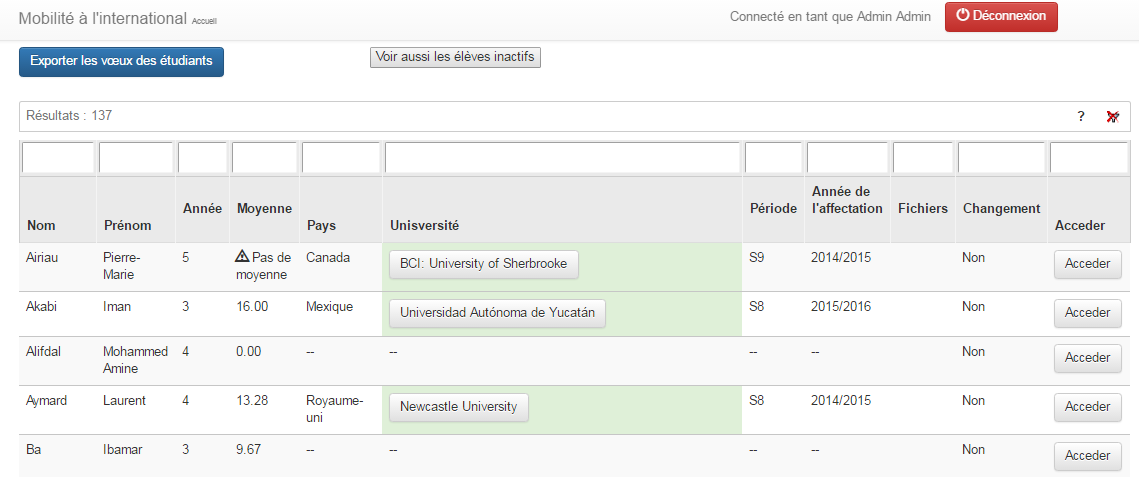
\includegraphics[scale=0.5]{images/accueil_admin.PNG}
	\caption{Page d'accueil pour les admins}
	\label{accueil_admins}
\end{figure}

La liste des étudiants (voir figure \ref{accueil_admins}) n'affichent plus les vœux, mais seulement l'université à laquelle un étudiant est affecté (quand il est affecté). l'admin peut accéder aux informations sur un étudiant grâce à un bouton, et peut ainsi voir les vœux et les réordonner. L'admin peut aussi exporter la liste des vœux au format CSV pour en disposer sous un autre format s'il le souhaite. Afin de ne pas surcharger la liste des élèves, ils ne sont plus affichés après 5 ans. On peut toutefois les voir grâce à un bouton.

Le site ne propose pas d'envoi de mail, mais permet de récupérer automatiquement les adresses mails des élèves affichés dans la liste (en prenant en compte les filtres appliqués).
\bigbreak
Pour les options des algorithmes d'affectations, nous avons opté pour deux solutions :
\begin{itemize}
	\item un algorithme (utilisé en INFO) qui prend un classement global alternant 4A et 3A (premier de 4A, suivit du premier de 3A, puis le second de 4A etc),
	\item un algorithme (utilisé ailleurs) qui donne la priorité aux élèves de 4A lors de l'affectation.
\end{itemize}

Ces deux solutions satisfont les exigences des départements que nous avons rencontrés. De plus, les responsables RI ont toujours la main pour affecter manuellement des élèves, comme décrit dans le rapport précédent.

Au sujet des contrats d'études, les admins pourront désormais voir le précédent (s'il y en avait un), dans le cas où un élève en soumettrait un nouveau. S'il en refuse un, l'admin peut aussi laisser un commentaire expliquant ce qu'il faut corriger dans le contrat d'étude.

\section{Liste des universités}
Le fonctionnement de la liste des universités est celui décrit dans le rapport de spécifications fonctionnelles. Les admins peut désormais aussi supprimer une université s'il le souhaite (supprimant les vœux et affectations par la même occasion, bien que cette action demande une confirmation.

Nous n'avons néanmoins développé l'ajout de commentaires sur les universités par les admins et les élèves de retour de mobilité. Cela est du à un manque de temps et à l'avis des élèves interrogés, nous disant qu'ils seraient plutôt intéressés par un système de \textit{Wiki} pour chaque université.